\section{Apêndice}
\renewcommand{\thefigure}{A\arabic{figure}}
\renewcommand{\thetable}{A\arabic{table}}
\setcounter{figure}{0}
%------------------------------------------------------%
\subsection{(R4) Causalidade} %{{

Como já foi referido, para averiguar a causalidade do sistema foram colocadas duas entradas iguais até ao instante \(t_0\) e confirmou-se que as saídas do sistema para os pares de sinais eram iguais até ao mesmo instante \(t_0\).

Dentro destas condições foram testados bastantes sinais de entrada e analisadas as respetivas saídas. Salientam-se alguns pares de sinais testados na seguinte tabela: 

%\iffalse
\begin{table}[h!]
\caption{Pares de sinais de entrada testados no âmbito da causalidade.}
\label{tab:table1}
\centering
    \begin{tabular}{||c | c||} 
        \hline
        \underline{\textbf{Sinal 1}} & \underline{\textbf{Sinal 2}} \\ [0.5ex] 
        \hline\hline
        \((t+2) \cdot u(t-t_0)\) & \(\sin(t) \cdot u(t-t_0)\) \\ [0.5ex]
        \hline
        \(t^2 \cdot u(-t+t_0) + 2u(t-t_0)\) & \(t^2 \cdot u(-t+t0)+e^t \cdot u(t-t_0)\) \\ [0.5ex]
        \hline
        \(0 \cdot t \equiv 0\) & \(u(t+t_0)-u(t-t_0)\) \\ [0.5ex]
        \hline
        \(t^2-1\) & \((t^2-1) \cdot u(-t+t_0)\) \\ [0.5ex]
        \hline
        \(\cos[\frac{\pi}{2} \cdot u(-t+t_0)]\) & \(0 \cdot t \equiv 0 \) \\ [0.5ex] 
        \hline
        \(\sin[u(t-t_0) \cdot t]\) & \(\cos[\frac{\pi}{2} \cdot u(-t+t_0)]\) \\ [0.5ex]
        \hline
        \(e^{\sin[u(t-t_0) \cdot t]}\) & \(\cos[\frac{\pi}{2} \cdot u(t-t_0)]\) \\ [0.5ex]
        \hline
    \end{tabular}
\end{table}
%\fi

Para diferentes valores de \(t_0 \in \mathbb{Z}\) entre -10 e 10.

%\iffalse
\begin{figure}[H] 
    \begin{subfigure}[b]{0.5\linewidth}
        \centering
        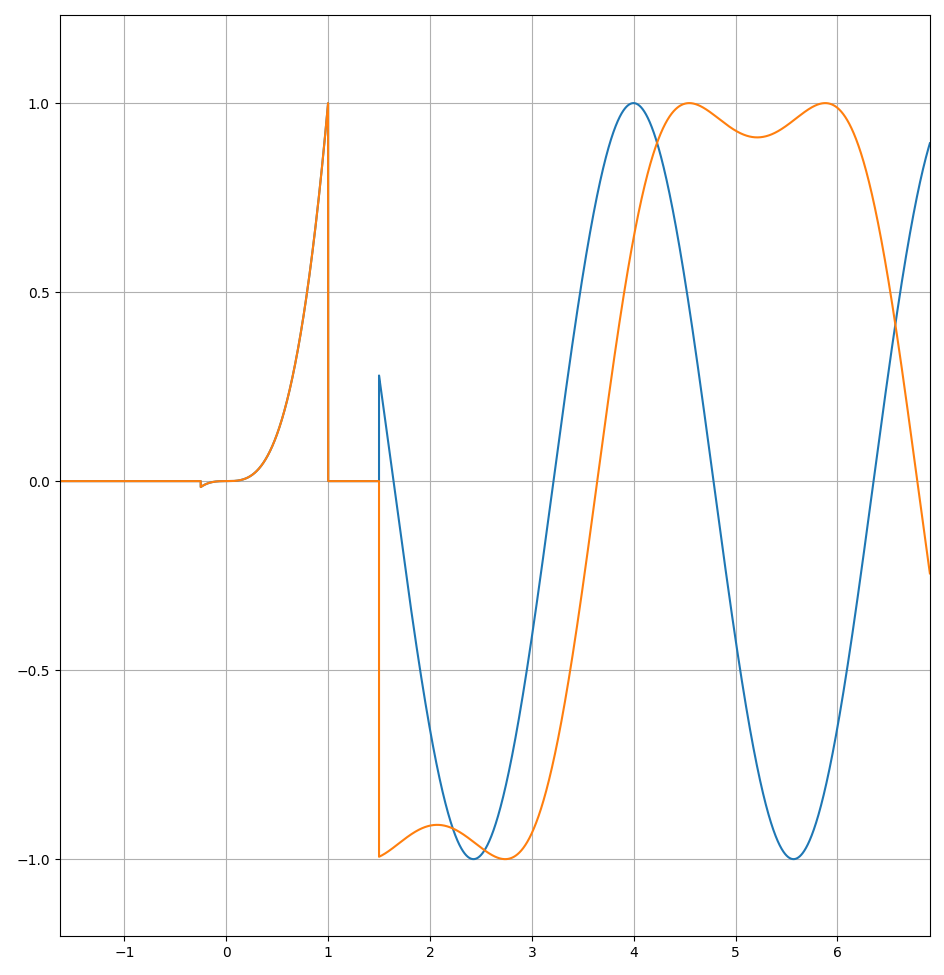
\includegraphics[width=0.6\linewidth]{prints/par_1.png}
        \caption{1\textordmasculine\ par com \(t_0 = 1\).} 
        \label{fig:par_1} 
        %%\vspace{4ex}
    \end{subfigure}%% 
    \begin{subfigure}[b]{0.5\linewidth}
        \centering
        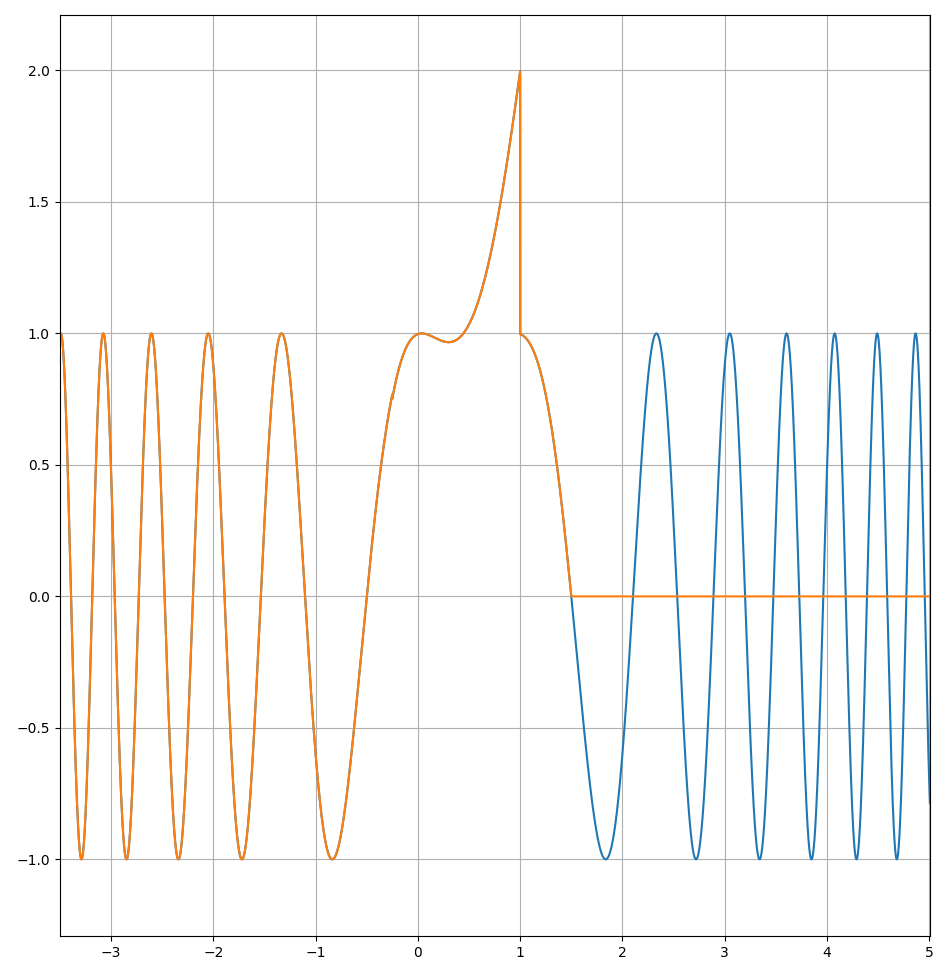
\includegraphics[width=0.6\linewidth]{prints/par_4.png} 
        \caption{4\textordmasculine\ par com \(t_0 = 1\).} 
        \label{fig:par_4} 
        %%\vspace{4ex}
    \end{subfigure} 
        \begin{subfigure}[b]{0.5\linewidth}
        \centering
        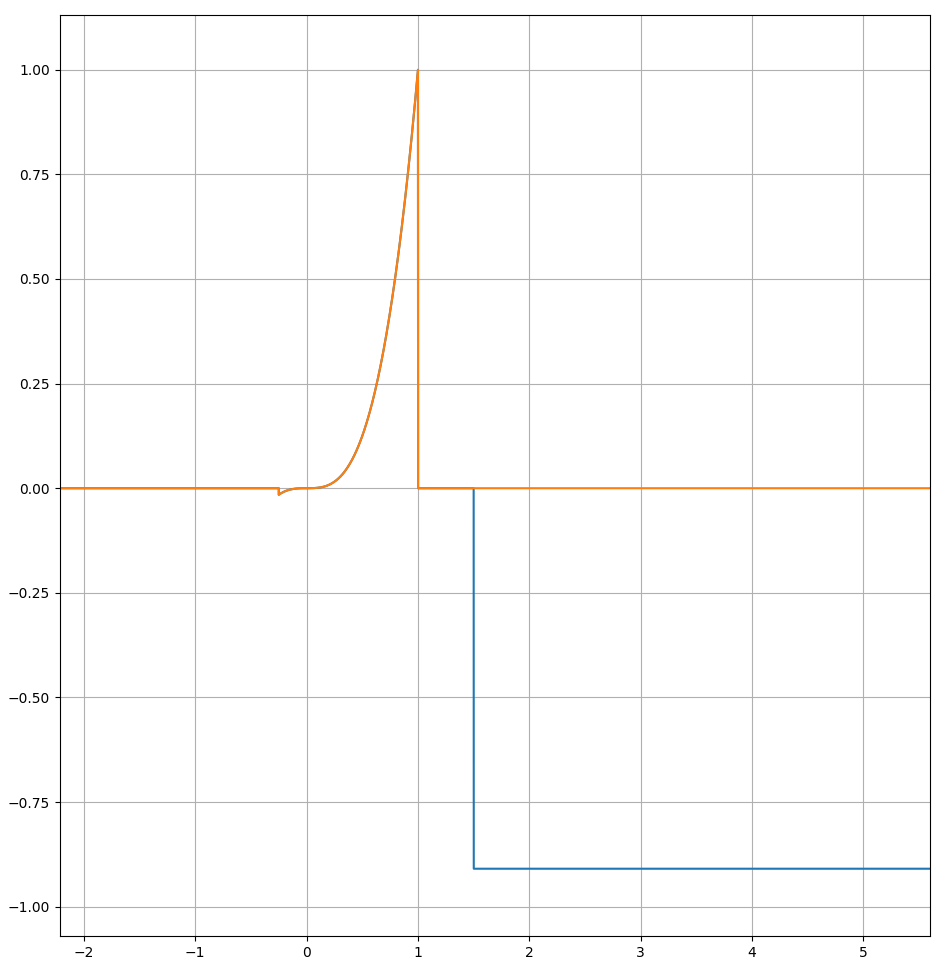
\includegraphics[width=0.6\linewidth]{prints/par_5.png}
        \caption{5\textordmasculine\ par com \(t_0 = 1\).} 
        \label{fig:par_5} 
        %%\vspace{4ex}
    \end{subfigure}%% 
    \begin{subfigure}[b]{0.5\linewidth}
        \centering
        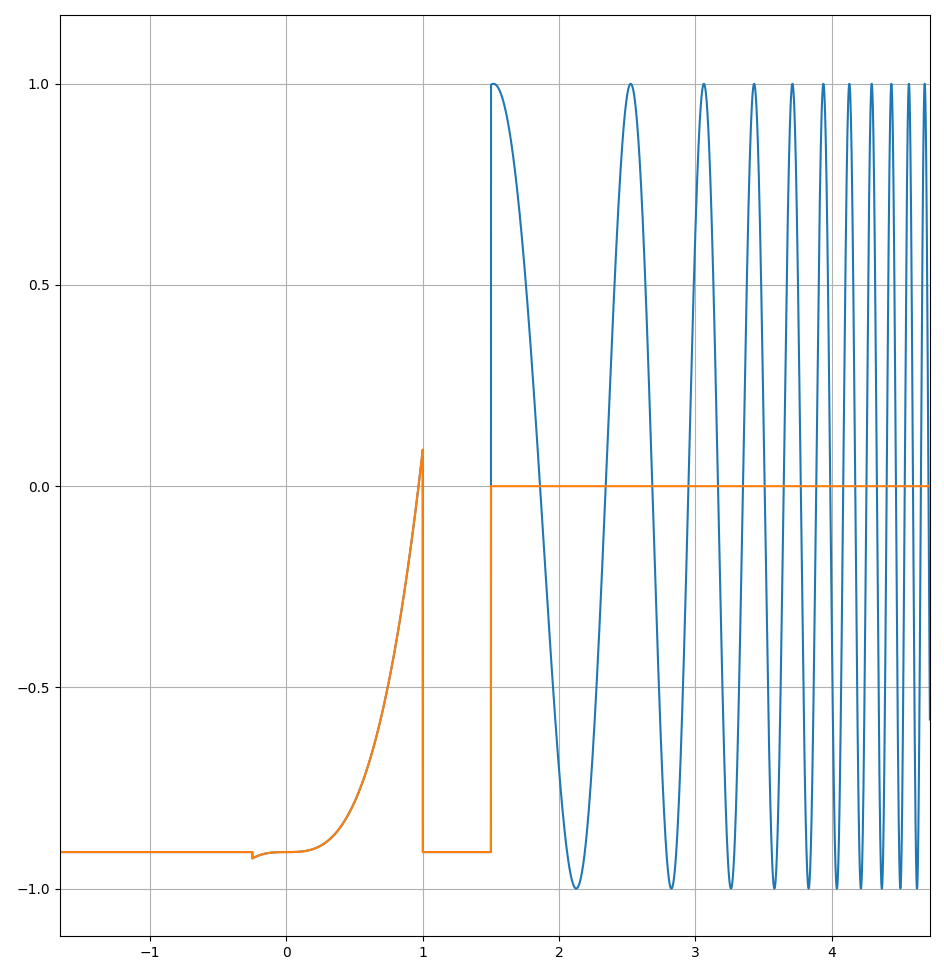
\includegraphics[width=0.6\linewidth]{prints/par_7.png} 
        \caption{7\textordmasculine\ par com \(t_0 = 1\).} 
        \label{fig:par_7} 
        %%\vspace{4ex}
    \end{subfigure}
    \caption{Respostas do \(sistema_2\) a alguns pares da \hyperref[tab:table1]{Tab. 1}.}
    \label{fig:appendix_A.1}
\end{figure}
%\fi

%}}
\clearpage
%------------------------------------------------------%
\subsection{(R5) Estabilidade} %{{

Como referido na discussão principal, para averiguar a estabilidade do sistema foram testados sinais de entradas limitados e observou-se que as saídas do sistema para estes sinais também eram limitadas.

Eis alguns exemplos pertinentes: \( \sin(\frac{1}{t}) \), \( [\cos(2t)]^2 \), \( (1+e^t) \cdot u(-t) \), \( 5e^{-2t} \cdot u(t-2) \), \( t^2 \cdot (u(t+2) - u(t-4)) \), \( \frac{\sin(5t)}{5t} \), \(u(t+1)-u(t-1)\)...

%\iffalse
\begin{figure}[H] 
    \begin{subfigure}[b]{0.5\linewidth}
        \centering
        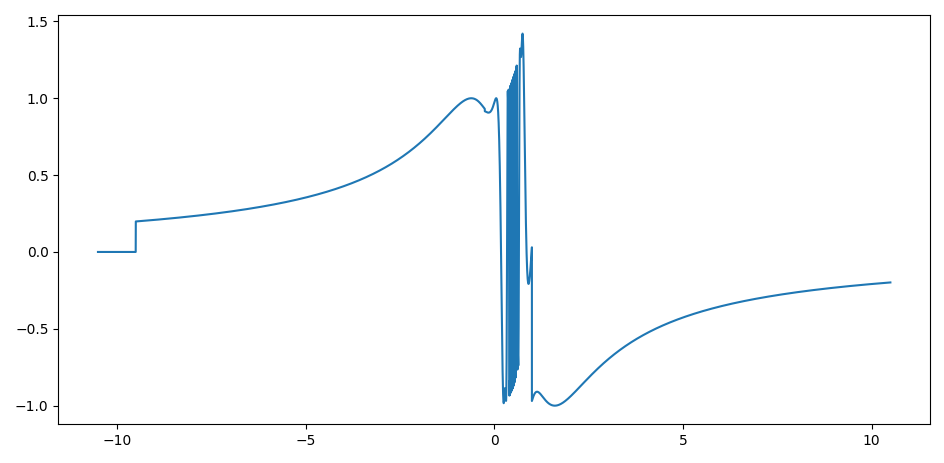
\includegraphics[width=1\linewidth]{prints/exemplo_1.png}
        \caption{\( \sin(\frac{1}{t}) \xleftrightarrow[]{\ sistema_2\ } y_1\).} 
        \label{fig:exemplo1} 
        %%\vspace{4ex}
    \end{subfigure}%% 
    \begin{subfigure}[b]{0.5\linewidth}
        \centering
        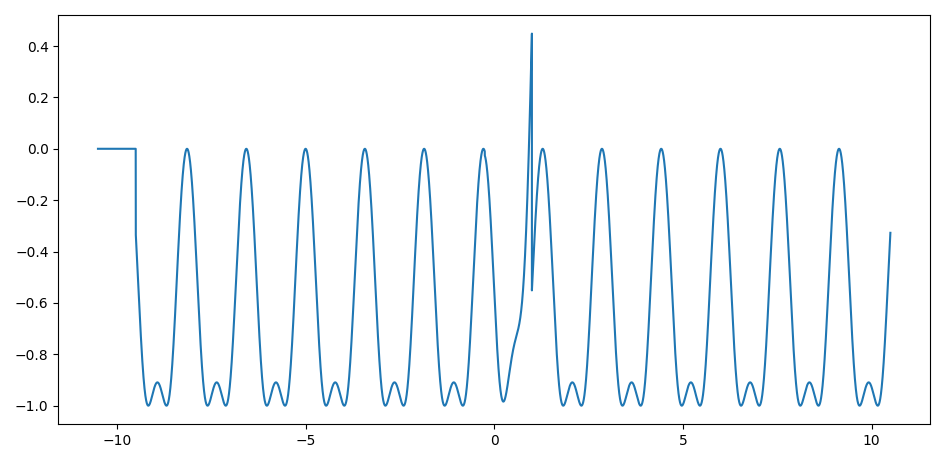
\includegraphics[width=1\linewidth]{prints/exemplo_2.png} 
        \caption{\( [\cos(2t)]^2 \xleftrightarrow[]{\ sistema_2\ } y_2\).} 
        \label{fig:exemplo2} 
        %%\vspace{4ex}
    \end{subfigure} 
        \begin{subfigure}[b]{0.5\linewidth}
        \centering
        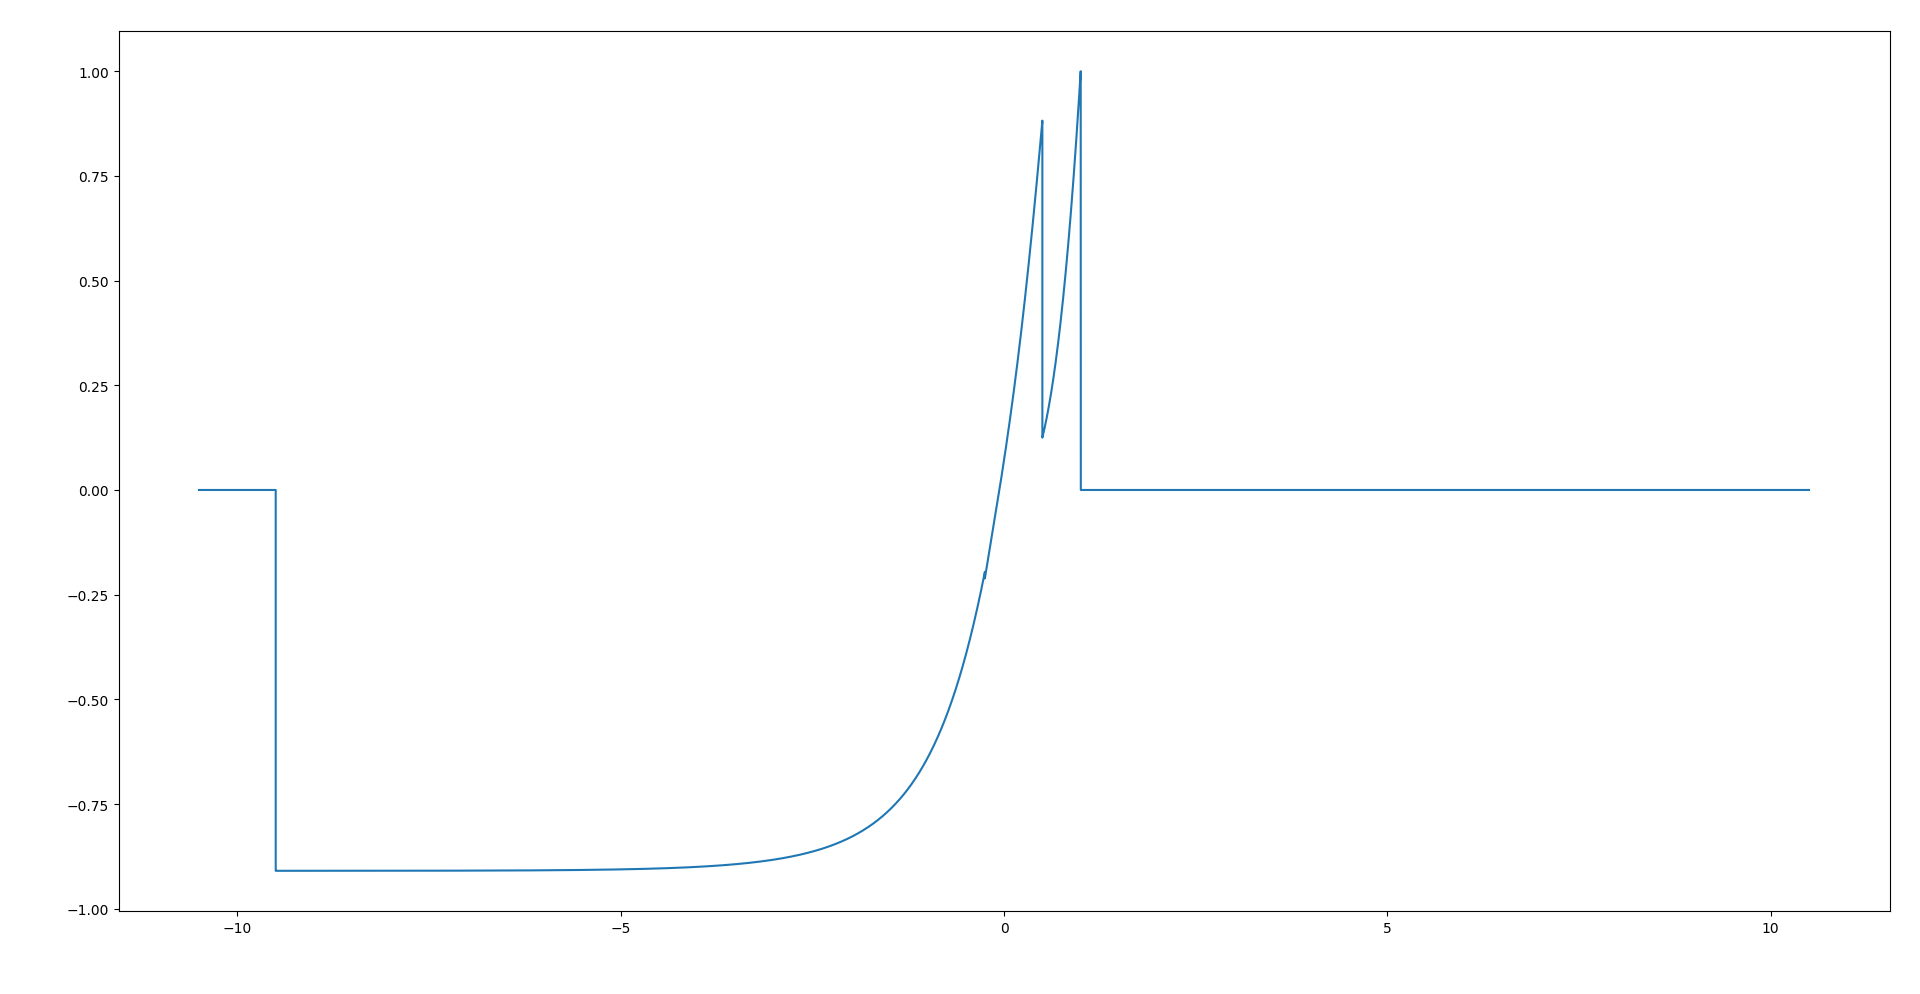
\includegraphics[width=1\linewidth]{prints/exemplo_3.png}
        \caption{\( (1+e^t) \cdot u(-t) \xleftrightarrow[]{\ sistema_2\ } y_3\).} 
        \label{fig:exemplo3} 
        %%\vspace{4ex}
    \end{subfigure}%% 
    \begin{subfigure}[b]{0.5\linewidth}
        \centering
        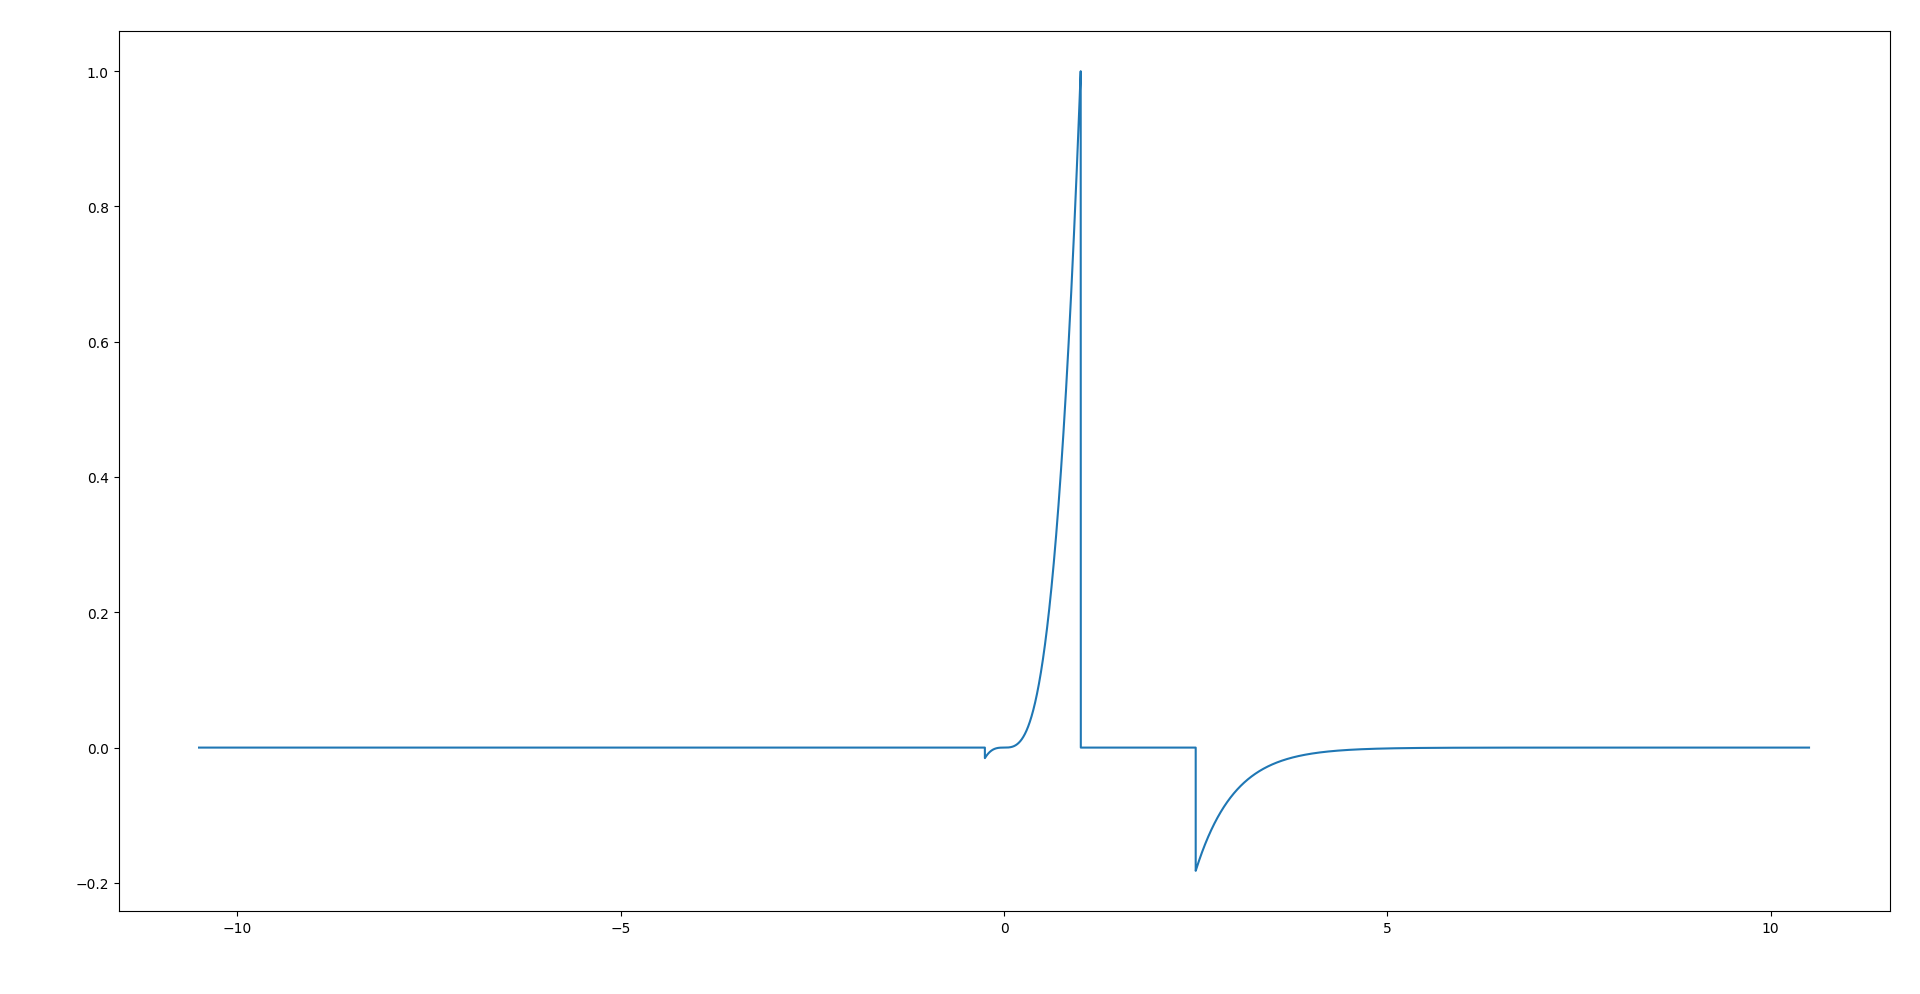
\includegraphics[width=1\linewidth]{prints/exemplo_4.png} 
        \caption{\( 5e^{-2t} \cdot u(t-2) \xleftrightarrow[]{\ sistema_2\ } y_4\).} 
        \label{fig:exemplo4} 
        %%\vspace{4ex}
    \end{subfigure}
    \begin{subfigure}[b]{0.5\linewidth}
        \centering
        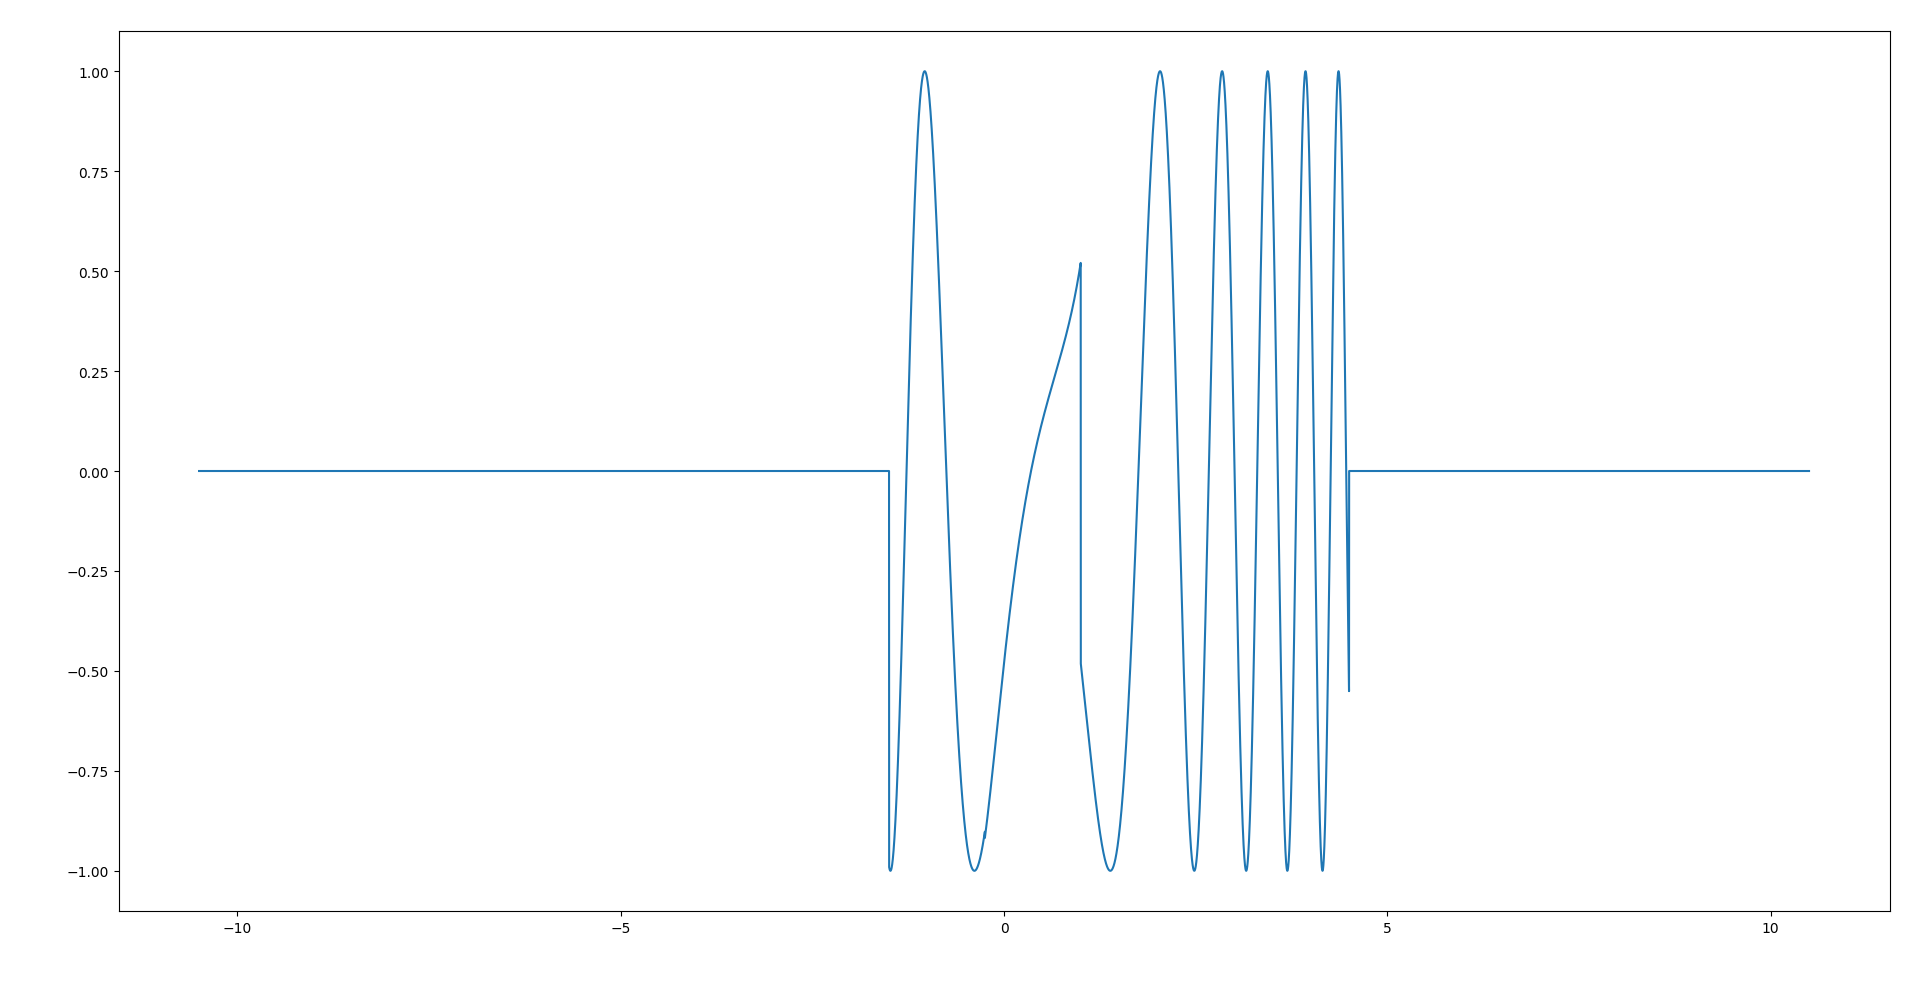
\includegraphics[width=1\linewidth]{prints/exemplo_5.png}
        \caption{\( t^2 \cdot (u(t+2) - u(t-4)) \xleftrightarrow[]{\ sistema_2\ } y_5\).} 
        \label{fig:exemplo5} 
        %%\vspace{4ex}
    \end{subfigure}%% 
    \begin{subfigure}[b]{0.5\linewidth}
        \centering
        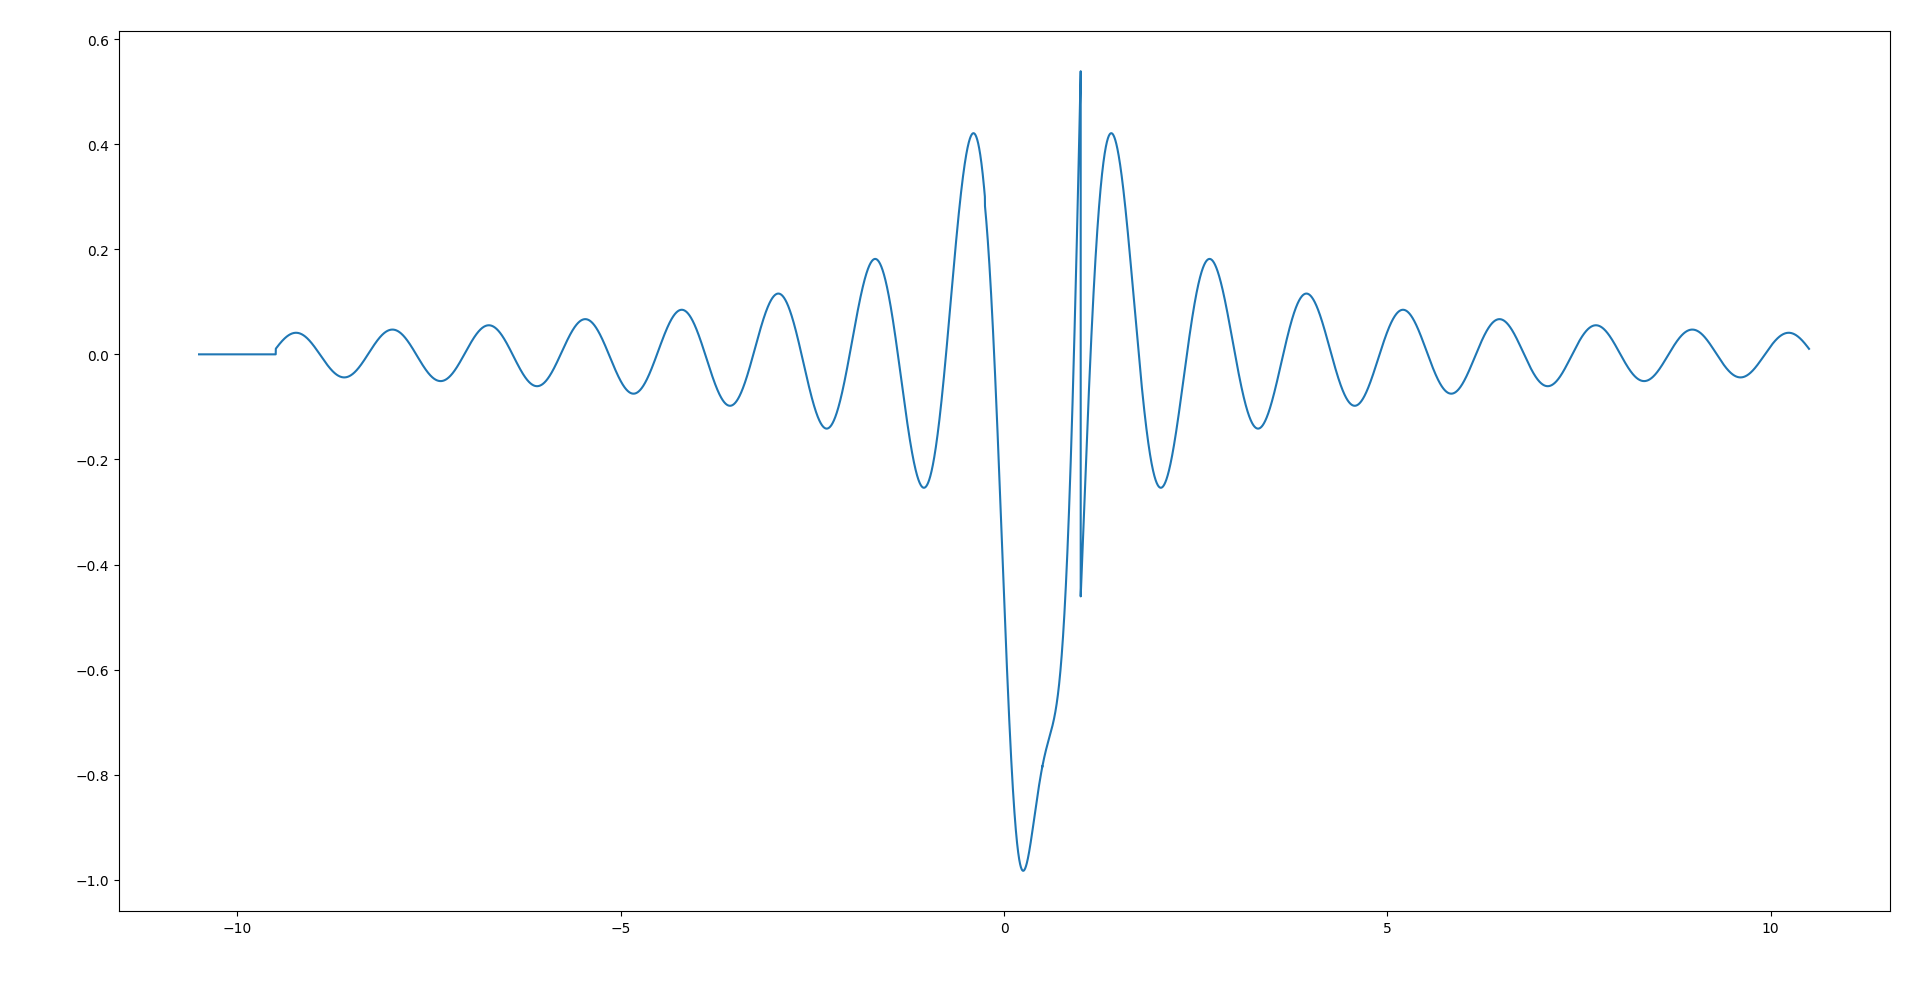
\includegraphics[width=1\linewidth]{prints/exemplo_6.png} 
        \caption{\( \frac{\sin(5t)}{5t} \xleftrightarrow[]{\ sistema_2\ } y_6\).} 
        \label{fig:exemplo6} 
        %%\vspace{4ex}
    \end{subfigure} 
    \begin{subfigure}[b]{0.5\linewidth}
        \centering
        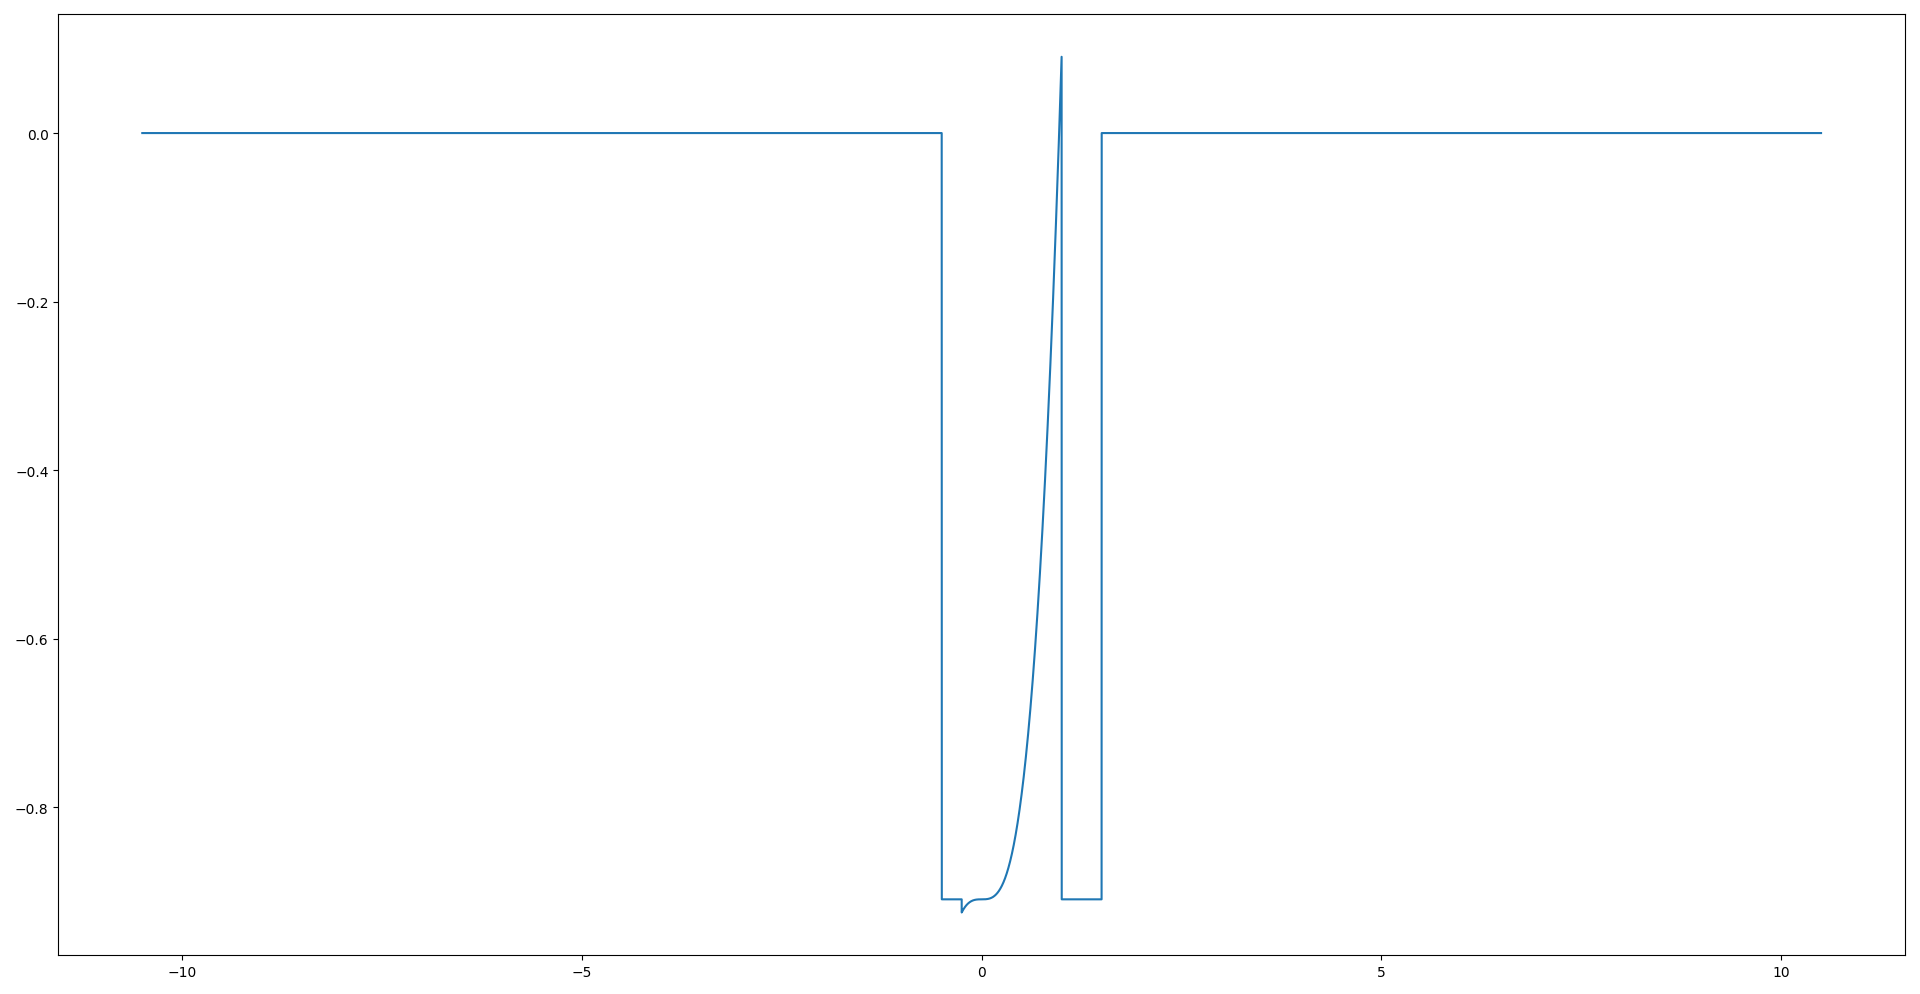
\includegraphics[width=1\linewidth]{prints/exemplo_7.png} 
        \caption{\( u(t+1)-u(t-1) \xleftrightarrow[]{\ sistema_2\ } y_7\).} 
        \label{fig:exemplo7} 
        %%\vspace{4ex}
    \end{subfigure} 
    \centering
    \caption{Resposta do \(sistema_2\) ao sinais limitados enumerados.}
    \label{fig:appendix_A.2}
\end{figure}
%\fi

%}}
\clearpage
%------------------------------------------------------%
\subsection{(R6) Resposta em frequência} %{{

\begin{normalsize}
\underline{1. Metodo (Sinais e Sistemas)} 
\vspace{0.25cm}
\end{normalsize}

Vamos então obter os valores de \(h(t)\) e \(\mathcal{H}(j\omega)\) teoricamente.
Tendo em conta que temos um circuito RC é fácil obter o ganho do circuito através do uso de impedâncias:
\[ y(t) = \frac{\frac{1}{j\omega C}}{R + \frac{1}{j\omega C}} \cdot x(t) \iff y(t) = \frac{1}{j\omega RC + 1} \cdot x(t) \]

Com este resultado é fácil concluir que o ganho do sistema é dado por

\[ \mathcal{H}(j\omega) = \frac{1}{j\omega RC+1} \]

Com o valor da resposta do sistema em frequência, obtém-se a resposta em tempo, \(h(t)\), calculando a \(\mathcal{TF}^{-1}\{\mathcal{H}(j\omega)\}\). Como sabemos que:

\[ e^{-at}u(t)\xleftrightarrow[]{\mathcal{TF}} \frac{1}{a+j\omega} \]

É fácil, então, de deduzir a  \(\mathcal{TF}^{-1}\{\mathcal{H}(j\omega)\}\), uma vez que

\[ \mathcal{H}(j\omega) = \frac{1}{RC} \frac{1}{\frac{1}{RC}+j\omega} \xleftrightarrow[]{\mathcal{TF}^{-1}} h(t)= \frac{1}{RC}e^{-\frac{1}{RC}t}u(t) \]

Concluímos portanto as expressões utilizadas na questão (R6):

\[ h(t) = \frac{1}{RC}e^{\frac{-t}{RC}} \cdot u(t)\text{,}\ \forall t \]

\[ \mathcal{H}(j\omega) = \frac{1}{1 + j\omega RC}\text{,}\ \forall \omega \]

%\iffalse
\begin{normalsize}
    \begin{flushleft}
        \underline{2. Metodo alternativo (Análise de Circuitos)} 
    \end{flushleft}
\end{normalsize}

Ora, suponhamos que o nosso sinal de entrada, \(x(t) = u(t)\), representa a fonte de tensão do circuito. Aplicando a Lei de Kirchhoff das correntes, temos que 

\[ \frac{u(t)}{R} + C \cdot y'(t) = 0\text{,} \]

uma equação diferencial ordinária de primeira ordem bastante conhecida, cuja solução é simplesmente:

\[ y(t) = y(+\infty) + [y(0^+) - y(+\infty)]e^{\frac{-t}{RC}} \iff y(t) = 1 - e^{\frac{-t}{RC}}\text{,}\ \forall t \geq 0 \]

Logo, temos que \(y(t) = 1 - e^{\frac{-t}{RC}} = u(t) * h(t)\). Como queremos a resposta do sistema ao impulso unitário, derivamos y(t) em t:

\[  y'(t) = (\frac{du}{dt} * h)(t) = (\delta * h)(t) = h(t) \iff h(t) = \frac{1}{RC}e^{\frac{-t}{RC}} \text{,}\ \forall t \geq 0 \]

\[ \therefore h(t) = \frac{1}{RC}e^{\frac{-t}{RC}} \cdot u(t)\text{,}\ \forall t \]

Deste modo, fazendo o sinal de entrada do sistema \(x(t) = \delta(t)\) e aplicando \(\mathcal{TF}\{.\}(j\omega)\) a \(y(t) = h(t)\), deduzimos a resposta do sistema ao impulso unitário, no domínio da frequência (i.e., \(H(j\omega)\)).

\[ \mathcal{TF}\{h(t)\}(j\omega) = H(j\omega) = \frac{1}{1 + j\omega RC}\text{,}\ \forall \omega \]
%\fi

%}}
%------------------------------------------------------%